% !Mode:: "TeX:UTF-8"
% UTF-8 编辑器
\chapter{插图样本}
\setcounter{subsubsection}{0} %将计数器subsubsection置零
\section{单图排列 \label{chap5:figure1}}
\begin{figure}[ht]
\centering
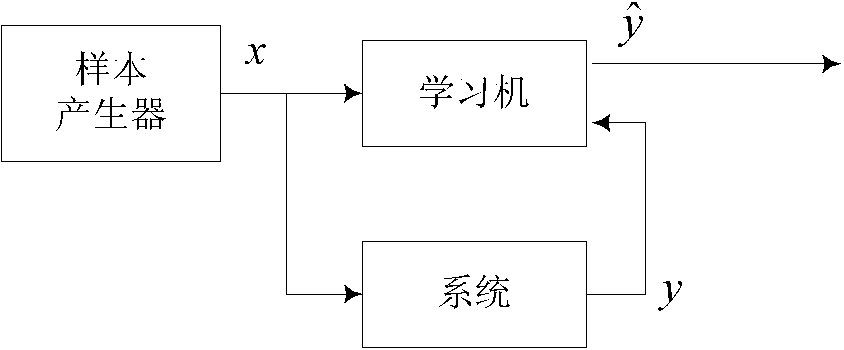
\includegraphics[totalheight=1in]{learn.pdf}
\caption{学习机的结构框图} \label{fig:7-1}
\end{figure}
如图\ref{fig:7-1}所示:
\section{图形并置 \label{chap5:figure2}}
对于比较小的图形我们希望把两个并排放在一起浮动, 且将 \verb/\includegraphics/
命令放到小页环境(miniipage)中可以让用户更好地控制图形的对齐方式.

例如图\ref{fig:7-2}是仅带一个浮动标题的二图并置.
\begin{figure}[ht]
  \centering
  \begin{minipage}[c]{0.5\textwidth}
    \centering
    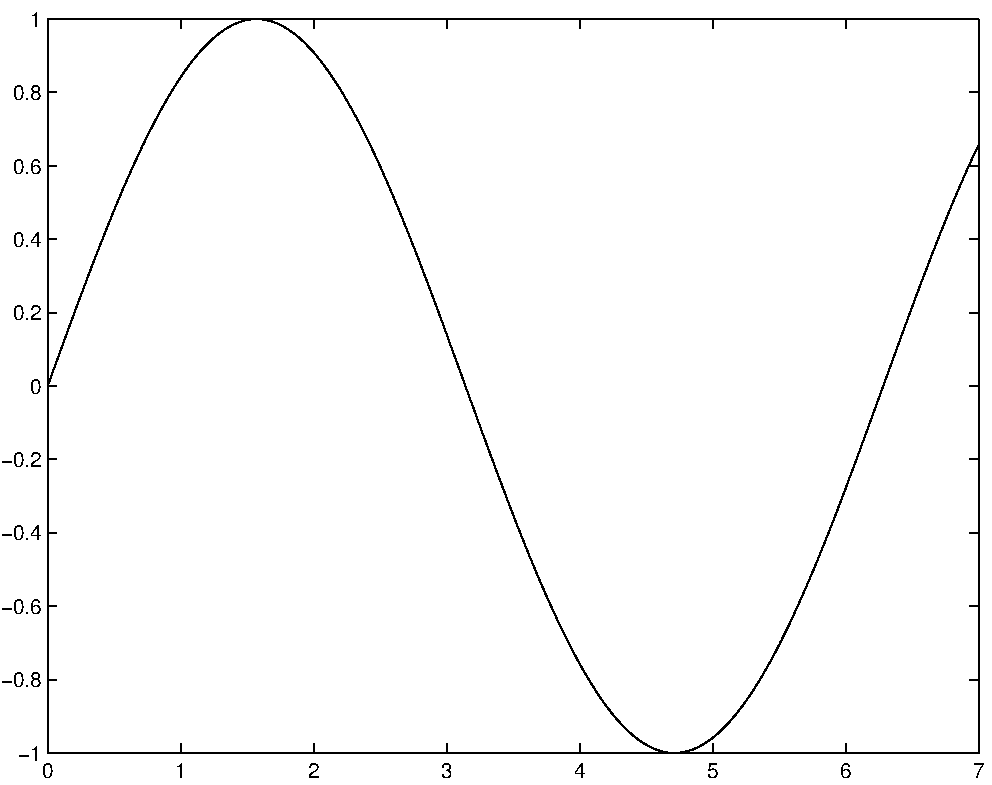
\includegraphics[width=5cm,height=3cm]{sine.pdf}
  \end{minipage}%
  \begin{minipage}[c]{0.5\textwidth}
    \centering
    \includegraphics[width=4cm,height=3cm]{Learn.pdf}
  \end{minipage}
  \caption{采用同个活动标题\label{fig:7-2}}
\end{figure}


下面产生的两图也并列(图\ref{fig:float2-1}和图\ref{fig:float2-2}), 但是有各自的图形标题.
\begin{figure}[ht]
\begin{minipage}[t]{0.45\linewidth}
\centering
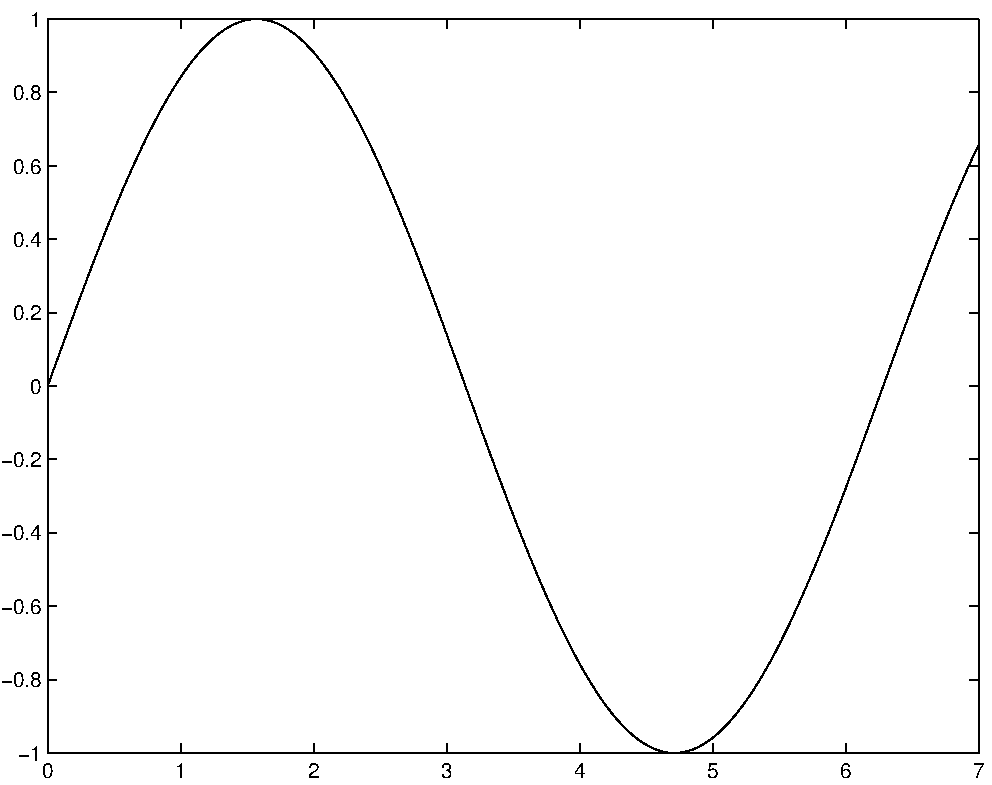
\includegraphics[width=5cm,height=3cm]{sine.pdf}
\caption{这是第一个图\label{fig:float2-1}}
\end{minipage}%
\hfill
\begin{minipage}[t]{0.5\linewidth}
\centering
\includegraphics[width=5cm,height=3cm]{Learn.pdf}
\caption{这是第二个图\label{fig:float2-2}}
\end{minipage}
\end{figure}


下面产生的图\ref{mini:subfigs}有二个子图(图\ref{fig:float3-1}和图\ref{fig:float3-2})组成一组,
而其中的每一幅图又保持其相对独立性.

\begin{figure}[t]
  \centering
  \subfigure[这是第一个图\label{fig:float3-1}]{
    \label{mini:suba} %% label for first subfigure
    \begin{minipage}[b]{0.4\textwidth}
      \centering
      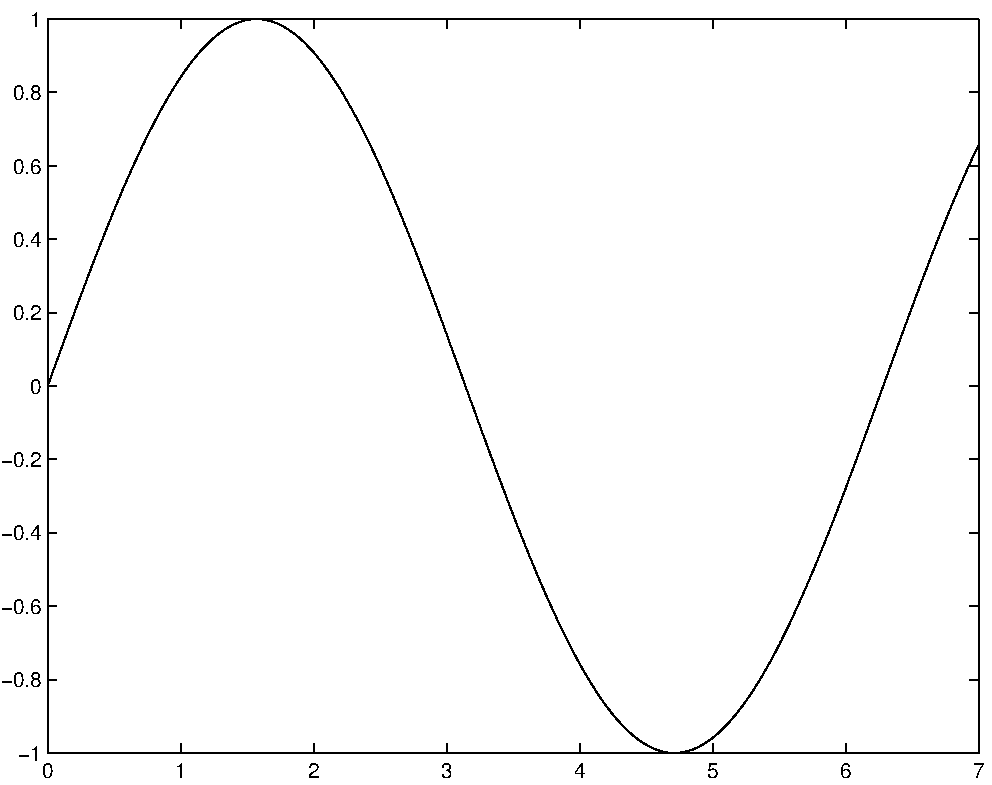
\includegraphics[width=1.5in]{sine.pdf}
    \end{minipage}}%
  \subfigure[这是第一个图\label{fig:float3-2}]{
    \label{mini:subb} %% label for second subfigure
    \begin{minipage}[b]{0.4\textwidth}
      \centering
      \includegraphics[width=1.5in]{Learn.pdf}
    \end{minipage}}
  \caption{二个图形并置}
  \label{mini:subfigs} %% label for entire figure
  \vspace{0.5\textheight}
\end{figure}

